\section{Wstęp} % (fold)
  \label{sec:wstep}

  Zadaniem projektowym było zaimplementowanie oraz zbadanie skuteczności
  algorytmu ewolucyjnego dla jednoprocesorowego problemu szeregowania zadań,
  gdzie kryterium była minimalizacja sumy ważonej czasów opóźnień.

% section wstep (end)

\section{Opis problemu} % (fold)
  \label{sec:problem}

  Problem szeregowania zadań na jednym procesorze z minimalizacją sumy ważonej
  czasów opóźnień można zdefiniować w następujący sposób.
  \vspace{1em}

  Danych jest $n$ zadań, z których każde zadanie $i$ jest dostępne w chwili $t=0$
  oraz wymaga $p_i > 0$ jednostek czasu na wykonanie, posiada oczekiwany termin
  zakończenia $d_i > 0$ oraz priorytet $w_i > 0$. Zadanie $i$ jest opóźnione,
  gdy czas zakończenia zadania $C_i > d_i$, a miarą opóźnienia zadania $i$
  jest $T_i = \max(0, C_i - d_i)$. Należy znaleźć taką kolejność wykonywania
  zadań, aby zminimalizować kryterium $TWT = \sum_{i = 1}^{n} w_i \cdot T_i$.

% section problem (end)

\section{Opis algorytmu} % (fold)
  \label{sec:algorytm}

  Algorytm genetyczny należy do grupy algorytmów heurystycznych i jest oparty
  na zjawisku ewolucji biologicznej. Algorytmy te często wykorzystuje się do
  rozwiązywania problemów NP-trudnych. Zwykle robi się tak ze względu na to, że
  czas odnalezienie rozwiązania optymalnego jest zbyt duży, a wystarczająco
  dobrym może być rozwiązanie przybliżone.
  \vspace{1em}

  Działanie algorytmu można podzielić na następujące etapy.
  \begin{enumerate}
    \item Generowanie populacji początkowej;
    \item \label{start} Wybierz elitę na podstawie funkcji dopasowania;
    \item Stwórz nowe osobniki na podstawie selekcji rodziców z elity;
    \item Z określonym prawdopodobieństwem zmutuj niektóre z nowych osobników;
    \item Jeśli nowe osobniki nie są tak liczne, jak populacja początkowa,
          dołącz elitę do nowej populacji;
    \item Jeśli nie przekroczono zadanej liczby kroków, wróć do
          punktu~\ref{start}.
  \end{enumerate}
  \vspace{1em}

  Warto zwrócić uwagę, że osobnik należący do elity w algorytmie genetycznym
  może przetrwać bardzo wiele pokoleń, co w rzeczywistości nie jest możliwe.
  \vspace{1em}

  Wybór populacji początkowej został zrealizowany poprzez generowanie losowych
  permutacji zadań, a wybór rodziców uwarunkowany jest wynikiem funkcji
  przystosowania osobników.
  \vspace{1em}

  Jako algorytm mutacji użyty został losowy ruch typu invert. Zajście mutacji
  jest opisane pewnym, małym, prawdopodobieństwem i ma zachodzić niezwykle
  rzadko.
  \vspace{1em}

  Do krzyżowania osobników wykorzystany został operator PMX, który działa w
  następujący sposób.
  \begin{enumerate}
    \item Wybierz dwa różne punkty krzyżowania od $1$ do $n$, gdzie $n$ jest
          długością permutacji;
    \item Utwórz listę dwuelementowych wektorów permutacji na podstawie list
          wyciętych z permutacji rodziców;
    \item W każdym z rodziców zamień wszystkie elementy występujące na pozycji
          pierwszej w wektorze na elementy występujące na pozycji drugiej i
          odwrotnie.
  \end{enumerate}

% section algorytm (end)

\section{Implementacja} % (fold)
  \label{sec:impl}

  Algorytm zaimplementowany został w języku Erlang. Warto zwrócić uwagę, że
  język ten nie posiada takich konstrukcji jak pętle, a zmienne po przypisaniu
  do nich wartości nie mogą zostać zmodyfikowane. Komunikacja między procesami
  opiera się na wysyłaniu wiadomości, co jest to zaletą w przypadku,
  gdy język ten używany jest w aplikacjach wielowątkowych, gdyż w wielu
  przypadkach pozwala to na uniknięcie blokad.
  \vspace{1em}

  Funkcja dopasowania została zaimplementowana w następujący sposób.
  Funkcja \texttt{lists:foldl} wykonuje funkcję podaną jako pierwszy argument na
  liście podanej jako ostatni argument i zwraca wartość akumulatora, którego
  początkowy stan jest przekazany jako drugi argument. Pojedyncze zadanie jest
  reprezentowane jako krotka w formacie \texttt{\{Pj, Wj, Dj\}}. Funkcja
  dopasowania jest jedyną funkcją, która wymusza taki format zapisu danych, a
  więc zmieniając tę jedną funkcję można przystosować algorytm do rozwiązywania
  innego problemu.
  \singlespacing
  \begin{center}
  \begin{minted}[gobble=4]{erlang}
    fitness(Permutation) ->
      {_, Result} = lists:foldl(fun compute_fitness/2, {0, 0}, Permutation),
      Result.

    compute_fitness({Pj, Wj, Dj}, {Time, Acc}) ->
      {Time + Pj, Wj*max(0, Time + Pj - Dj) + Acc}.
  \end{minted}
  \end{center}
  \onehalfspacing
  \vspace{1em}

  Wybór pierwszej populacji zrealizowany został algorytmem losowym. Funkcja ta
  została zaimplementowana przy użyciu rekurencji ogonowej. Każdy osobnik w
  populacji reprezentuje określona permutacja zadań zapisana jako lista. Funkcja
  \texttt{spawn\_population} zwraca listę list, czyli listę osobników. W
  implementacji widać również wykorzystanie jednej z cech języków funkcyjnych,
  czyli dopasowywanie do wzorca, dzięki czemu nie zostało użyte żadne wyrażenie
  warunkowe.
  \singlespacing
  \begin{center}
  \begin{minted}[gobble=4]{erlang}
    spawn_population(Tasks, N) -> spawn_population(Tasks, N, []).
    spawn_population(_, 0, Acc) -> Acc;
    spawn_population(Tasks, N, Acc) ->
      Permutation = lists:keysort(2, [{X, random:uniform()} || X <- Tasks]),
      New = [X || {X,_} <- Permutation],
      spawn_population(Tasks, N - 1, [New|Acc]).
  \end{minted}
  \end{center}
  \onehalfspacing
  \vspace{1em}

  Implementacja algorytmu PMX została podzielona na trzy części. W pierwszej z
  nich wybierane są punkty krzyżowania, w drugiej generowane są wektory
  wykorzystywane przy krzyżowaniu, a w trzeciej wykonywana jest sama operacja
  krzyżowania.
  \singlespacing
  \begin{center}
  \begin{minted}[gobble=4]{erlang}
    breed(Parents = {P1, P2}, ProbabilityOfMutation) ->
      S1 = random:uniform(length(P1)),
      S2 = random:uniform(length(P2)),
      case S1 > S2 of
        true  -> breed(Parents, S2, S1, ProbabilityOfMutation);
        false -> breed(Parents, S1, S2, ProbabilityOfMutation)
      end.

    breed(Parents = {P1, P2}, S1, S2, P) ->
      V = breed_vector(Parents, S1, S2),
      C1 = lists:map(fun(X) -> lists:foldl(fun breed_swap/2, X, V) end, P1),
      C2 = lists:map(fun(X) -> lists:foldl(fun breed_swap/2, X, V) end, P2),
      {mutate(C1, P), mutate(C2, P)}.

    breed_swap({Gene, NewGene}, Gene) -> NewGene;
    breed_swap({Gene, NewGene}, NewGene) -> Gene;
    breed_swap({_, _}, Gene) -> Gene.

    breed_vector({Parent1, Parent2}, S1, S2) ->
      L1 = lists:sublist(Parent1, S1, S2 - S1),
      L2 = lists:sublist(Parent2, S1, S2 - S1),
      lists:zip(L1, L2).
  \end{minted}
  \end{center}
  \onehalfspacing
  \vspace{1em}

  Za główną pętlę algorytmu odpowiada funkcja \texttt{evolve}. To w niej
  dokonywany jest podział populacji na elitę oraz wybranie rodziców dla nowych
  pokoleń. Dodatkowym parametrem jest również znane rozwiązanie optymalne i
  jeśli zostanie ono osiągnięte wcześniej, algorytm przerywa swoje działanie.
  \singlespacing
  \begin{center}
  \begin{minted}[gobble=4]{erlang}

    evolve(Population, TimeLeft, Pmutation, Best) ->
      Sorted = sort_by_fitness(Population),
      evolve(Sorted, TimeLeft, Pmutation, hd(Sorted), Best).

    evolve(_, 0, _, BestSolution, _) -> {BestSolution, 0};
    evolve(Population, TimeLeft, Pmutation, _, Best) ->
      Length = length(Population) div 3,
      {Good, Bad} = lists:split(Length, Population),
      NewGood = reproduce(Good, Pmutation),
      Sorted = sort_by_fitness(NewGood ++ Good ++ lists:sublist(Bad, Length)),
      BestSolution = hd(Sorted),
      case fitness(BestSolution) =< Best of
        false -> evolve(Sorted, TimeLeft - 1, Pmutation, BestSolution, Best);
        true  -> {BestSolution, TimeLeft}
      end.
  \end{minted}
  \end{center}
  \onehalfspacing
  \vspace{1em}

  Tworzenie nowych osobników populacji odbywa się w funkcji \texttt{reproduce}.
  Wywołuje ona funkcję \texttt{breed} dla każdej z par rodziców.
  \singlespacing
  \begin{center}
  \begin{minted}[gobble=4]{erlang}
    reproduce(Generation, P) -> reproduce(Generation, [], P).
    reproduce([], NewGeneration, _) -> NewGeneration;
    reproduce([P1, P2|Rest], NewGeneration, P) ->
      {C1, C2} = breed({P1, P2}, P),
      reproduce(Rest, [C1, C2|NewGeneration], P);
    reproduce([Last], NewGeneration, P) ->
      reproduce([], [Last|NewGeneration], P).
  \end{minted}
  \end{center}
  \onehalfspacing
  \vspace{1em}

  Za mutacje odpowiada funkcja \texttt{mutate}. Została zaimplementowana tak,
  aby osobnik był modyfikowany tylko z pewnym prawdopodobieństwem
  $(\frac{1}{2})^\textrm{P}$ w zależności od przekazywanego parametru.
  \singlespacing
  \begin{center}
  \begin{minted}[gobble=4]{erlang}
    mutate(Permutation, P) ->
      case probability(P) of
        true  -> mutate(Permutation);
        false -> Permutation
      end.

    mutate(Permutation) ->
      S1 = random:uniform(length(Permutation)),
      S2 = random:uniform(length(Permutation)),
      case S1 > S2 of
        true  -> mutate(Permutation, S2, S1);
        false -> mutate(Permutation, S1, S2)
      end.

    mutate(Permutation, S1, S2) ->
      {Head, Tail} = lists:split(S1, Permutation),
      {Middle, End} = lists:split(S2 - S1, Tail),
      Head ++ lists:reverse(Middle) ++ End.
  \end{minted}
  \end{center}
  \onehalfspacing
  \vspace{1em}

  Algorytm zwraca najlepsze znalezione rozwiązanie oraz liczbę generacji, która
  pozostała, która jest różna od zera, jeśli rozwiązanie optymalne udało znaleźć
  się wcześniej.
% section impl (end)

\section{Testy i wyniki} % (fold)
  \label{sec:testy}

  Testy zostały przeprowadzone na serwerze wyposażonym w procesor Intel Xeon
  L5520 pracujący z częstotliwością 2.27GHz oraz 512MB pamięci RAM. Program
  został uruchamiany przez wirtualną maszynę Erlanga w wersji R14B.
  \vspace{1em}

  W programie istnieje możliwość regulowania takich parametrów, jak rozmiar
  populacji, ilość kroków oraz prawdopodobieństwo mutacji. Testy zostały
  przeprowadzone dla populacji o wielkościach 50, 100 oraz 200 osobników oraz
  dla 1000, 5000 oraz 10000 kroków. Jako ostatni parametr została przekazana
  liczba 4, co oznacza, że prawdopodobieństwo mutacji wynosiło $\frac{1}{16}$.
  W tabelach użyte zostały następujące oznaczenia: S - ilość kroków, C - ilość
  osobników w instancji.
  \vspace{1em}

  \begin{table}[h!]
  \begin{center}
  \caption{Średnie wyniki dla instancji 40-elementowej.}
  \begin{tabular}{c|ccc}
    \hline
      S \textbackslash C & 50 & 100 & 200 \\
    \hline
      \multicolumn{4}{c}{Instancja 1, optimum = 913} \\
    \hline
      1000  & 1420 & 1269 & 1230 \\
      5000  & 1183 & 1195 & 1191 \\
      10000 & 1238 & 1150 & 1261 \\
    \hline
      \multicolumn{4}{c}{Instancja 2, optimum = 16225} \\
    \hline
      1000  & 17533 & 17510 & 17206 \\
      5000  & 17224 & 17308 & 17134 \\
      10000 & 17403 & 17261 & 17036
  \end{tabular}
  \end{center}
  \end{table}

  \begin{table}[h!]
  \begin{center}
  \caption{Średnie wyniki dla instancji 50-elementowej.}
  \begin{tabular}{c|ccc}
    \hline
      S \textbackslash C & 50 & 100 & 200 \\
    \hline
      \multicolumn{4}{c}{Instancja 1, optimum = 1996} \\
    \hline
      1000  & 2581 & 2313 & 2294 \\
      5000  & 2345 & 2332 & 2118 \\
      10000 & 2255 & 2180 & 2187 \\
    \hline
      \multicolumn{4}{c}{Instancja 2, optimum = 26276} \\
    \hline
      1000  & 29794 & 28893 & 28105 \\
      5000  & 28910 & 28106 & 27971 \\
      10000 & 28654 & 28921 & 26550
  \end{tabular}
  \end{center}
  \end{table}

  \begin{table}[h!]
  \begin{center}
  \caption{Średnie wyniki dla instancji 100-elementowej.}
  \begin{tabular}{c|ccc}
    \hline
      S \textbackslash C & 50 & 100 & 200 \\
    \hline
      \multicolumn{4}{c}{Instancja 1, optimum = 5988} \\
    \hline
      1000  & 11777 & 10422 & 8204 \\
      5000  & 8801  & 7690  & 7743 \\
      10000 & 8707  & 7831  & 7693 \\
    \hline
      \multicolumn{4}{c}{Instancja 2, optimum = 58258} \\
    \hline
      1000  & 84880 & 75768 & 70093 \\
      5000  & 73886 & 69868 & 68674 \\
      10000 & 73324 & 70162 & 69181
  \end{tabular}
  \end{center}
  \end{table}

  \begin{table}[h!]
  \begin{center}
  \caption{Średni błąd dla instancji 40-elementowej.}
  \begin{tabular}{c|ccc}
    \hline
      S \textbackslash C & 50 & 100 & 200 \\
    \hline
      \multicolumn{4}{c}{Instancja 1, optimum = 913} \\
    \hline
      1000  & 0,55 & 0,39 & 0,35 \\
      5000  & 0,30 & 0,31 & 0,30 \\
      10000 & 0,36 & 0,26 & 0,38 \\
    \hline
      \multicolumn{4}{c}{Instancja 2, optimum = 16225} \\
    \hline
      1000  & 0,08 & 0,08 & 0,06 \\
      5000  & 0,06 & 0,07 & 0,06 \\
      10000 & 0,07 & 0,06 & 0,05
  \end{tabular}
  \end{center}
  \end{table}

  \begin{table}[h!]
  \begin{center}
  \caption{Średni błąd dla instancji 50-elementowej.}
  \begin{tabular}{c|ccc}
    \hline
      S \textbackslash C & 50 & 100 & 200 \\
    \hline
      \multicolumn{4}{c}{Instancja 1, optimum = 1996} \\
    \hline
      1000  & 0,29 & 0,16 & 0,15 \\
      5000  & 0,18 & 0,17 & 0,06 \\
      10000 & 0,13 & 0,09 & 0,10 \\
    \hline
      \multicolumn{4}{c}{Instancja 2, optimum = 26276} \\
    \hline
      1000  & 0,13 & 0,10 & 0,07 \\
      5000  & 0,10 & 0,07 & 0,06 \\
      10000 & 0,09 & 0,10 & 0,06
  \end{tabular}
  \end{center}
  \end{table}

  \begin{table}[h!]
  \begin{center}
  \caption{Średni błąd dla instancji 100-elementowej.}
  \begin{tabular}{c|ccc}
    \hline
      S \textbackslash C & 50 & 100 & 200 \\
    \hline
      \multicolumn{4}{c}{Instancja 1, optimum = 5988} \\
    \hline
      1000  & 0,97 & 0,74 & 0,37 \\
      5000  & 0,47 & 0,28 & 0,29 \\
      10000 & 0,45 & 0,31 & 0,28 \\
    \hline
      \multicolumn{4}{c}{Instancja 2, optimum = 58258} \\
    \hline
      1000  & 0,46 & 0,30 & 0,20 \\
      5000  & 0,27 & 0,20 & 0,18 \\
      10000 & 0,26 & 0,20 & 0,19
  \end{tabular}
  \end{center}
  \end{table}

  \begin{figure}[h!]
  \begin{center}
  \caption{Zależność dokładności wyniku od ilości kroków dla instancji z 40 zadaniami.}
  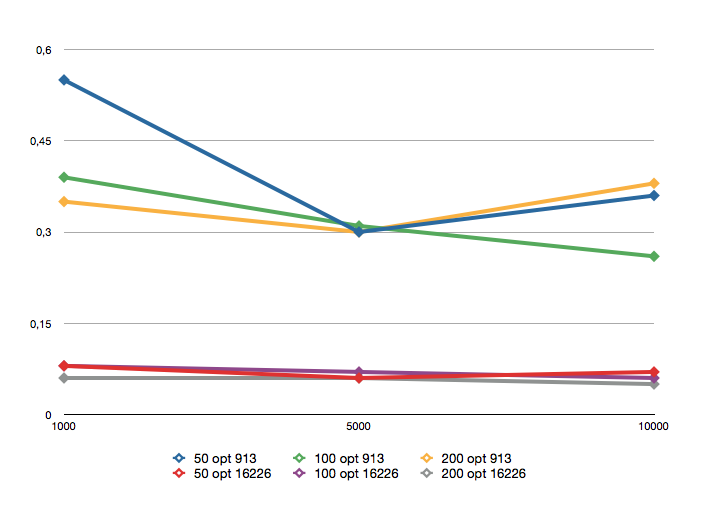
\includegraphics[scale=.6]{images/40.png}
  \end{center}
  \end{figure}

  \begin{figure}[h!]
  \begin{center}
  \caption{Zależność dokładności wyniku od ilości kroków dla instancji z 50 zadaniami.}
  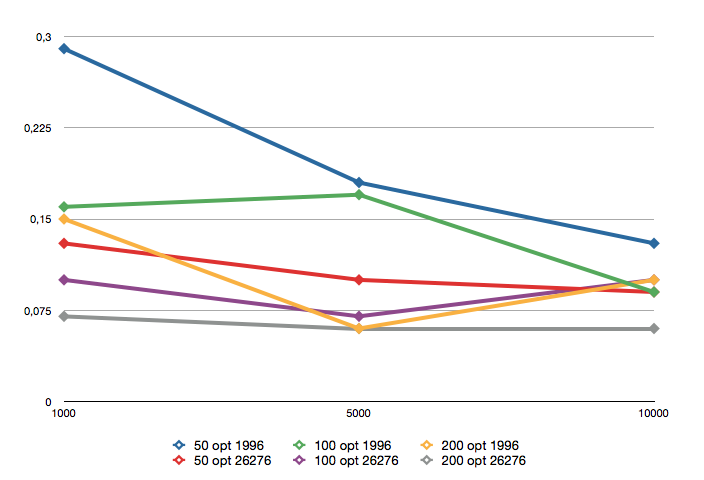
\includegraphics[scale=.6]{images/50.png}
  \end{center}
  \end{figure}

  \begin{figure}[h!]
  \begin{center}
  \caption{Zależność dokładności wyniku od ilości kroków dla instancji ze 100 zadaniami.}
  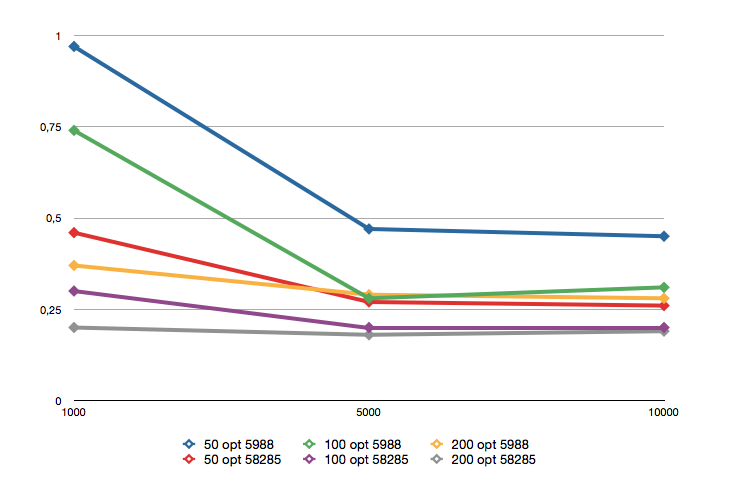
\includegraphics[scale=.6]{images/100.png}
  \end{center}
  \end{figure}

  \newpage
  W celu porównania algorytmów wyżarzania, tabu-search oraz algorytmu
  genetycznego obliczone zostały średnie wyniki dla danej instancji. Wyniki te
  oraz porównanie najgorszych i najlepszych rezultatów tych trzech algorytmów są
  przedstawione są na wykresach \ref{fig:cmp}, \ref{fig:min} oraz \ref{fig:max}.
  Wszystkie wykresy przedstawiają średni błąd w zależności od rozmiaru instancji.

  \begin{figure}[h!]
  \begin{center}
  \caption{Porównanie średnich wyników algorytmów.}
  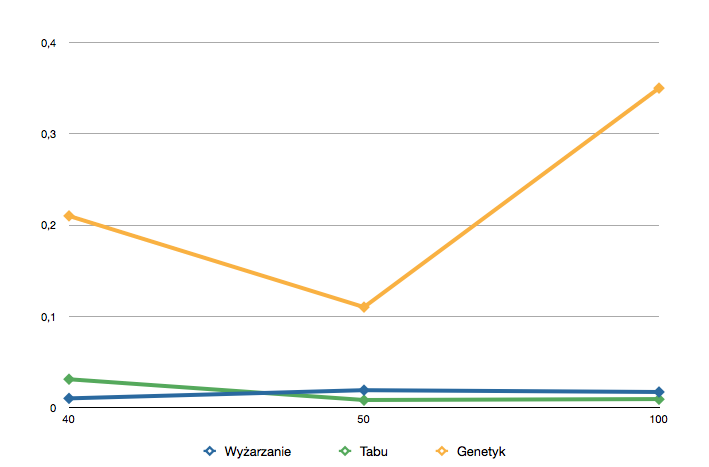
\includegraphics[scale=.6]{images/cmp.png}
  \label{fig:cmp}
  \end{center}
  \end{figure}

  \begin{figure}[h!]
  \begin{center}
  \caption{Porównanie najlepszych wyników algorytmów.}
  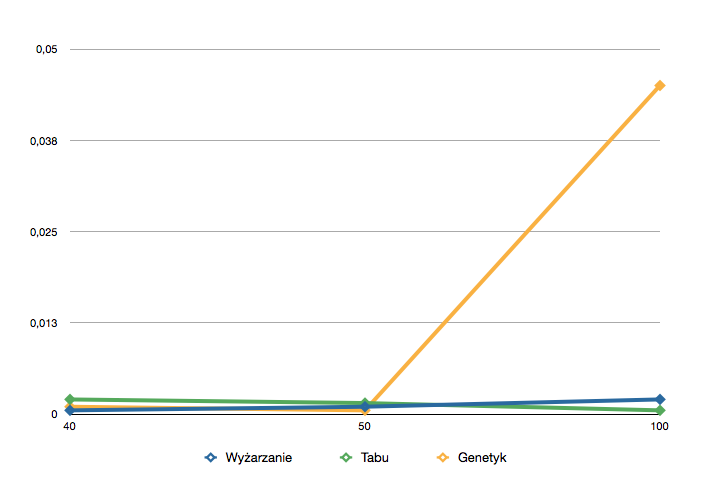
\includegraphics[scale=.6]{images/min.png}
  \label{fig:min}
  \end{center}
  \end{figure}

  \begin{figure}[h!]
  \begin{center}
  \caption{Porównanie najgorszych wyników algorytmów.}
  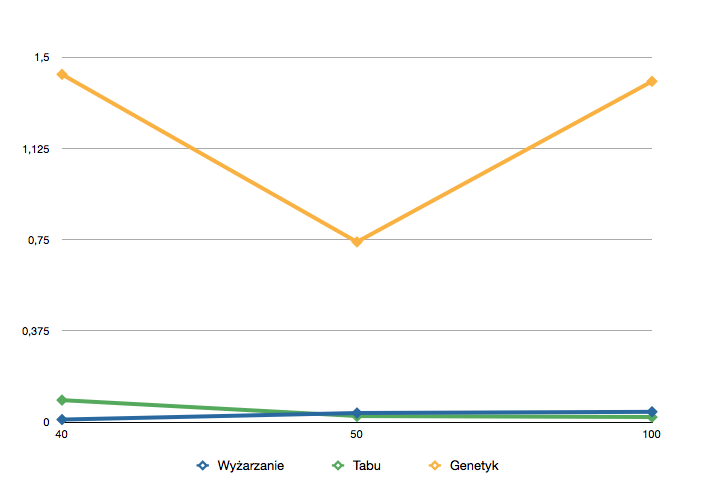
\includegraphics[scale=.6]{images/max.png}
  \label{fig:max}
  \end{center}
  \end{figure}

% section testy (end)
\newpage
\section{Wnioski} % (fold)
  \label{sec:wnioski}

  Dla większych instancji i tych samych parametrach algorytm genetyczny
  przegląda mniejszą część przestrzeni rozwiązań, co powoduje uzyskiwanie
  gorszych wyników. W takich wypadkach należałoby zwiększyć ilość kroków
  algorytmu, bądź też wielkość populacji, która również ma duże znaczenie dla
  wyników.
  \vspace{1em}

  Zwiększenie liczby osobników w populacji oraz ilości kroków powoduje, że
  algorytm jest w stanie odszukać lepsze rozwiązania, lecz dzieje się to kosztem
  czasu wykonywania algorytmu. Zmniejszenie tych parametrów przyspiesza
  działanie algorytmu, lecz owocuje kiepskimi wynikami. Sam program działał
  dosyć wolno, gdyż wymagał dużo kopiowania pamięci (sortowanie listy powoduje
  utworzenie nowej listy, a sam czas dostępu do $n$-tego elementu listy zajmuje
  $O(n)$). Dodatkowo warto zauważyć, że tak jak w przypadku tabu-search,
  wielkość instancji mam wpływ na czas działania algorytmu.
  \vspace{1em}

  W przeciwieństwie do algorytmu tabu, algorytm genetyczny zupełnie nie jest
  deterministyczny. Wynik w sporej części zależy od tego, jak dobra zostanie
  wylosowana populacja początkowa. W razie wylosowania kiepskiej populacji
  początkowej nie uda uzyskać się dobrego rozwiązania. Porównując wszystkie trzy
  algorytmy najlepsze wyniki dawał algorytm tabu-search, a najmniejszą złożoność
  obliczeniową ma algorytm wyżarzania, gdyż czas jego działania nie zależy od
  wielkości instancji.

% section wnioski (end)

\appendix
\section{Bibliografia} % (fold)
  \label{sec:biblio}
  \begin{enumerate}
    \item AI Techniques for Game Programming, Mat Buckland, The Premier Press, 2002
    \item \texttt{ftp://sith.ict.pwr.wroc.pl/Informatyka/PEA/ProjektPEA\_11\_12.pdf}
    \item \texttt{ftp://sith.ict.pwr.wroc.pl/Informatyka/PEA/genetyki.pdf}
  \end{enumerate}

% section biblio (end)
